\chapter{Perancangan}
\label{chap:perancangan}

Pada bab ini akan dijelaskan mengenai perancangan Sistem Informasi Riwayat
Mahasiswa yang akan dibuat. Mulai dari perancangan tampilan {\it web} yang digunakan,
perancangan modul, dan perancangan diagram sekuens.

\section{Perancangan Tampilan {\it Web} Yang Digunakan}
\label{sec:perancanganantarmuka}

Perancangan tampilan {\it web} yang akan dibuat untuk mengimplementasikan Sistem
Informasi Riwayat Mahasiswa terdapat tujuh buah perancangan yaitu halaman
awal, pilih mahasiswa, info mahasiswa, edit mahasiswa, lihat histori, lihat
versi ini dan entri baru.

\subsection{Tampilan Halaman Awal}
Perancangan tampilan {\it web} untuk halaman utama dapat dilihat pada
Gambar~\ref{fig:pilihmahasiswa}.

\begin{figure}[ht]
\centering
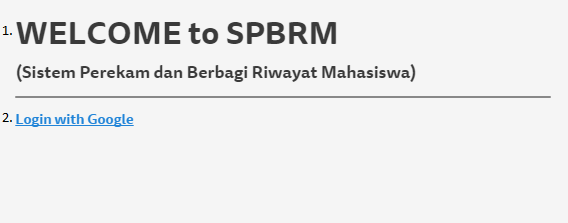
\includegraphics[scale=0.9]{Gambar/halamanawal.png}
\caption[Desain Antarmuka Halaman Awal]{Desain Antarmuka Halaman Awal}
\label{fig:halamanawal}
\end{figure}

Keterangan :
\begin{enumerate}[(1)]
\item
Bagian ini merupakan judul yang merupakan keterangan dari perangkat lunak.
\item
Bagian ini merupakan teks yang dapat diklik untuk melakukan login.
\end{enumerate}

\subsection{Tampilan {\it Web} Pilih Mahasiswa}
Perancangan tampilan {\it web} untuk pilih mahasiswa dapat dilihat pada
Gambar~\ref{fig:pilihmahasiswa}.

\begin{figure}[ht]
\centering
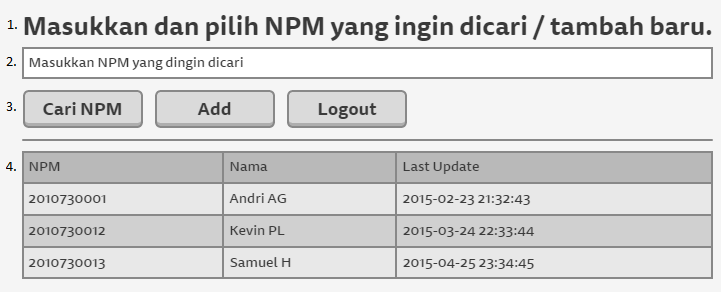
\includegraphics[scale=0.9]{Gambar/pilihmahasiswa.png}
\caption[Desain Antarmuka Pilih Mahasiswa]{Desain Antarmuka Pilih Mahasiswa}
\label{fig:pilihmahasiswa}
\end{figure}

Keterangan :
\begin{enumerate}[(1)]
\item
Bagian ini merupakan judul dari halaman untuk memilih mahasiswa.
\item
Bagian ini merupakan tombol untuk melakukan aksi add atau logout.
\item
Bagian ini merupakan tempat menampilkan data mahasiswa dalam bentuk tabel. NPM
dapat diklik untuk memilih mahasiswa.
\end{enumerate}

\subsection{Tampilan {\it Web} Info Mahasiswa}
Perancangan tampilan {\it web} untuk info mahasiswa dapat dilihat pada Gambar~\ref{fig:infomahasiswa}.
\begin{figure}[ht]
\centering
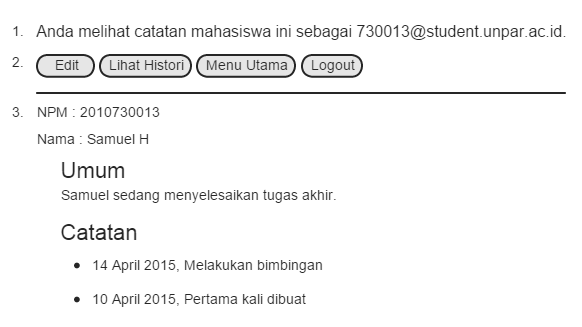
\includegraphics[scale=0.9]{Gambar/infomahasiswa.png}
\caption[Desain Antarmuka Info Mahasiswa]{Desain Antarmuka Info Mahasiswa}
\label{fig:infomahasiswa}
\end{figure}

Keterangan :
\begin{enumerate}[(1)]
\item
Bagian ini merupakan teks yang menampilkan keterangan dan juga pengguna yang sedang menggunakan Sistem Infomasi Riwayat Mahasiswa.
\item
Bagian ini merupakan tombol untuk melakukan aksi edit, lihat histori, pindah
ke menu utama, dan logout.
\item
Bagian ini merupakan tempat menampilkan info mahasiswa yang berasal dari database.
\end{enumerate}

\subsection{Tampilan {\it Web} Edit Mahasiswa}
Perancangan tampilan {\it web} untuk edit mahasiswa dapat dilihat pada Gambar~\ref{fig:editmahasiswa}.
\begin{figure}[ht]
\centering
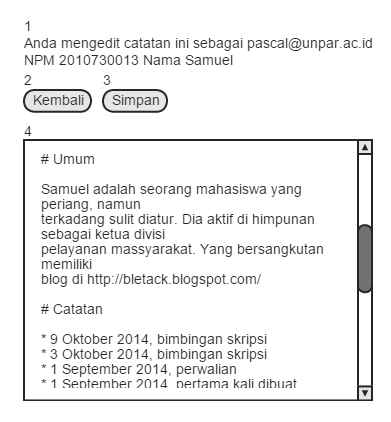
\includegraphics[scale=0.9]{Gambar/editmahasiswa.png}
\caption[Desain Antarmuka Edit Mahasiswa]{Desain Antarmuka Edit Mahasiswa}
\label{fig:editmahasiswa}
\end{figure}

Keterangan :
\begin{enumerate}[(1)]
\item
Bagian ini merupakan teks yang menampilkan keterangan dan juga pengguna yang
sedang menggunakan Sistem Infomasi Riwayat Mahasiswa.
\item
Bagian ini merupakan teks yang menampilkan NPM dan nama mahasiswa yang telah
dipilih untuk diedit.
\item
Bagian ini merupakan tombol untuk melakukan aksi kembali, simpan untuk perubahan
yang telah dilakukan, pindah ke menu utama, dan logout.
\item
Bagian ini merupakan tempat menampilkan catatan mahasiswa yang berasal dari
database dan dapat diedit (ditulis dengan format markdown).
\end{enumerate}

\subsection{Tampilan {\it Web} Lihat Histori}
Perancangan tampilan {\it web} untuk lihat histori dapat dilihat pada Gambar~\ref{fig:lihathistori}.
\begin{figure}[ht]
\centering
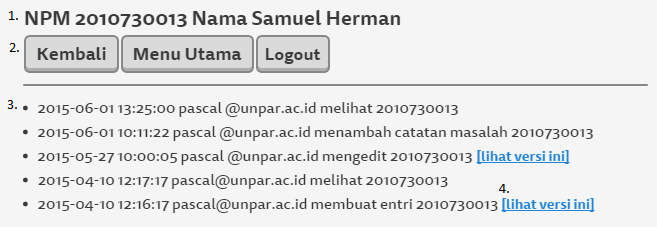
\includegraphics[scale=0.9]{Gambar/lihathistori.png}
\caption[Desain Antarmuka Lihat Histori]{Desain Antarmuka Lihat Histori}
\label{fig:lihathistori}
\end{figure}

Keterangan :
\begin{enumerate}[(1)]
\item
Bagian ini merupakan tombol untuk melakukan aksi kembali, pindah ke menu utama,
dan logout.
\item
Bagian ini merupakan teks yang menampilkan keterangan NPM dan nama mahasiswa
yang telah dipilih untuk dilihat historinya.
\item
Bagian ini merupakan daftar histori dari mahasiswa yang telah dipilih.
\end{enumerate}

\subsection{Tampilan {\it Web} Lihat Versi Ini}
Perancangan tampilan {\it web} untuk lihat versi ini dapat dilihat pada
Gambar~\ref{fig:lihatversiini}.
\begin{figure}[ht]
\centering
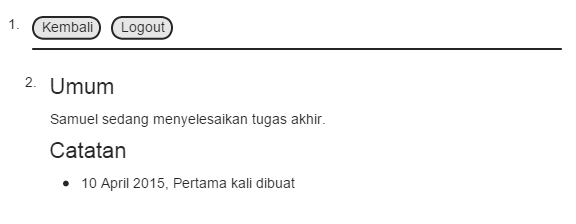
\includegraphics[scale=0.9]{Gambar/lihatversiini.png}
\caption[Desain Antarmuka Lihat Versi Ini]{Desain Antarmuka Lihat Versi Ini}
\label{fig:lihatversiini}
\end{figure}

Keterangan :
\begin{enumerate}[(1)]
\item
Bagian ini merupakan tombol untuk melakukan aksi kembali dan logout.	
\item
Bagian ini merupakan daftar histori dari mahasiswa yang telah dipilih.
\end{enumerate}

\subsection{Tampilan {\it Web} Entri Baru}
Perancangan tampilan {\it web} untuk entri baru dapat dilihat pada Gambar~\ref{fig:entribaru}.
\begin{figure}[ht]
\centering
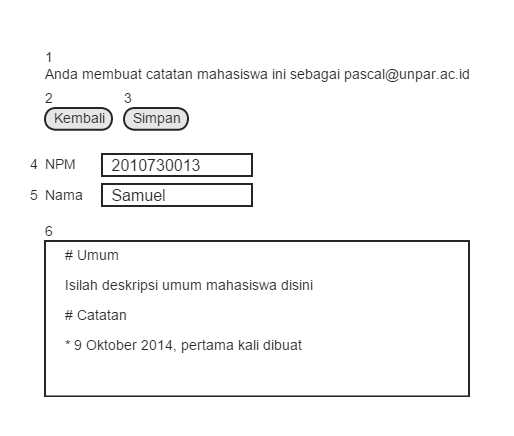
\includegraphics[scale=0.9]{Gambar/entribaru.png}
\caption[Desain Antarmuka Entri Baru]{Desain Antarmuka Pilih Entri Baru}
\label{fig:entribaru}
\end{figure}

Keterangan :
\begin{enumerate}[(1)]
\item
Bagian ini merupakan teks yang menampilkan keterangan dan juga pengguna yang
sedang menggunakan Sistem Infomasi Riwayat Mahasiswa.
\item
Bagian ini merupakan tombol untuk melakukan aksi kembali ke pilih mahasiswa,
simpan, menu utama, dan logout.
\item
Bagian ini merupakan form yang terdiri dari area untuk memasukkan NPM mahasiswa,
nama mahasiswa, dan keterangan mahasiswa yang akan ditambah dengan format yang
telah disediakan (ditulis dengan format markdown).
\end{enumerate}

\section{Perancangan Modul}
\label{sec:perancanganmodul}

Perancangan modul untuk sistem informasi riwayat mahasiswa yang akan dibuat
dapat dilihat pada sub bab berikut.

\subsection{Modul Login}
Modul login yang dilakukan oleh pengguna (dosen) dapat dilihat pada Tabel
\ref{tab:modullogin}.

\begin{table}[ht]
\centering
\caption[Tabel Modul Login]{Modul Login}
\label{tab:modullogin}
\begin{tabular}{|c|p{7cm}|}
\hline
Nama Modul & index.php\\
\hline
Input & {\it username}, {\it password}\\
\hline
Output & -\\
\hline
Tabel yang diakses & -\\
\hline
Deskripsi & Pengguna memasukkan {\it username} dan {\it password} kemudian
sistem akan melakukan autentikasi menggunakan Google Oauth.\\
\hline
\end{tabular}
\end{table}

\subsection{Modul Pilih Mahasiswa}
Modul pilih mahasiswa yang dilakukan oleh pengguna (dosen) dapat dilihat pada
Tabel \ref{tab:modulpilihmahasiswa}.

\begin{table}[ht]
\centering
\caption[Tabel Modul Pilih Mahasiswa]{Modul Pilih Mahasiswa}
\label{tab:modulpilihmahasiswa}
\begin{tabular}{|c|p{7cm}|}
\hline
Nama Modul & list.php\\
\hline
Input & npm\\
\hline
Output & Tabel mahasiswa\\
\hline
Tabel yang diakses & InfoMahasiswa\\
\hline
Deskripsi & Pengguna memilih npm yang ingin dicari sebagai input yang akan
diteruskan ke modul info mahasiswa dan pengguna juga dapat membaut entri baru.\\
\hline
\end{tabular}
\end{table}

\subsection{Modul Info Mahasiswa}
Modul info mahasiswa yang dilakukan oleh pengguna (dosen) dapat dilihat pada
Tabel \ref{tab:modulinfomahasiswa}.

\begin{table}[ht]
\centering
\caption[Tabel Modul Info Mahasiswa]{Modul Info Mahasiswa}
\label{tab:modulinfomahasiswa}
\begin{tabular}{|c|p{7cm}|}
\hline
Nama Modul & view.php\\
\hline
Input & -\\
\hline
Output & Info mahasiswa\\
\hline
Tabel yang diakses & InfoMahasiswa dan Histori\\
\hline
Deskripsi & Pengguna mendapatkan laporan barupa info mahasiswa yang telah
dipilih sebelumnya pada modul pilih mahasiswa. Pengguna dapat merubah info
mahasiswa yang ada dan dapat melihat histori setiap mahasiswa.\\
\hline
\end{tabular}
\end{table}

\subsection{Modul Edit Mahasiswa}
Modul {\it edit} mahasiswa yang dilakukan oleh pengguna (dosen) dapat dilihat
pada Tabel \ref{tab:moduleditmahasiswa}.

\begin{table}[ht]
\centering
\caption[Tabel Modul {\it Edit} Mahasiswa]{Modul {\it Edit} Mahasiswa}
\label{tab:moduleditmahasiswa}
\begin{tabular}{|c|p{7cm}|}
\hline
Nama Modul & edit.php\\
\hline
Input & teks dalam format markdown\\
\hline
Output & -\\
\hline
Tabel yang diakses & InfoMahasiswa dan Histori\\
\hline
Deskripsi & Pengguna memasukkan atau merubah keterangan mahasiswa pada teks area
yang telah disediakan menggunakan teks dengan sintaks Markdown lalu
pengguna menyimpan untuk menaruh perubahan yang dilakukan. Pengguna dapat
kembali ke modul info mahasiswa tanpa melakukan perubahan.\\
\hline
\end{tabular}
\end{table}

\subsection{Modul Lihat Histori}
Modul lihat histori yang dilakukan oleh pengguna (dosen) dapat dilihat pada
Tabel \ref{tab:modullihathistori}.

\begin{table}[ht]
\centering
\caption[Tabel Modul Lihat Histori]{Modul Lihat Histori}
\label{tab:modullihathistori}
\begin{tabular}{|c|p{7cm}|}
\hline
Nama Modul & history.php\\
\hline
Input & -\\
\hline
Output & Daftar histori mahasiswa\\
\hline
Tabel yang diakses & Histori\\
\hline
Deskripsi & Pengguna mendapatkan laporan berupa daftar hostori yang dimiliki
setiap mahasiswa.\\
\hline
\end{tabular}
\end{table}

\subsection{Modul Entri Baru}
Modul entri baru yang dilakukan oleh pengguna (dosen) dapat dilihat pada Tabel
\ref{tab:modulentribaru}.

\begin{table}[ht]
\centering
\caption[Tabel Modul Entri Baru]{Modul Entri Baru} 
\label{tab:modulentribaru}
\begin{tabular}{|c|p{7cm}|}
\hline
Nama Modul & new.php\\
\hline
Input & npm, nama, dan teks dalam format markdown\\
\hline
Output & -\\
\hline
Tabel yang diakses & InfoMahasiswa dan Histori\\
\hline
Deskripsi & Pengguna memasukkan npm, nama, dan keterangan mahasiswa pada teks
area yang telah disediakan menggunakan teks dengan sintaks Markdown lalu
pengguna menyimpan untuk membuat entri baru tersebut. Pengguna dapat kembali ke
modul pilih mahasiswa tanpa melakukan perubahan.\\
\hline
\end{tabular}
\end{table}

\section{Perancangan Diagram Relasional}
\label{sec:perancangandiagramrelasional}

Berdasarkan ERD pada sub sub bab 3.6.3, maka dapat dihasilkan perancangan diagram relasional yang dapat dilihat pada Gambar \ref{fig:diagramrelasional}.

\begin{figure}[ht]
\centering
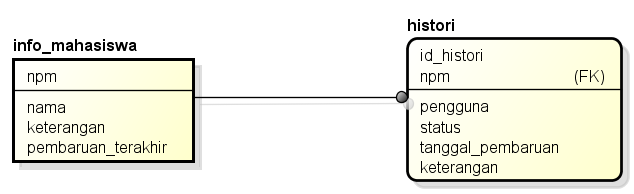
\includegraphics[scale=1]{Gambar/diagramrelasional.png}
\caption[Diagram Relasional]{Diagram Relasional} 
\label{fig:diagramrelasional}
\end{figure}

\section{Perancangan Tabel Sistem Informasi Riwayat Mahasiswa}
\label{sec:perancangantabel}

\subsection{Perancangan Tabel Info Mahasiswa}
Untuk rancangan tabel info mahasiswa dapat dilihat pada Tabel
\ref{tab:rancangantabelinfomahasiswa}.

\begin{table}[ht]
\caption[Tabel Rancangan Tabel Info Mahasiswa]{Rancangan Tabel Info Mahasiswa}
\label{tab:rancangantabelinfomahasiswa}
\centering
\begin{tabular}{|l|l|p{1.2cm}|p{1.2cm}|p{1.2cm}|l|}
\hline
Atribut & Tipe Data & Ukuran & Primary Key & Foreign Key & Keterangan\\
\hline
npm & varchar & 10 & yes & no & -\\
\hline
nama & varchar & 60 & no & no & -\\
\hline
keterangan & text & - & no & no & -\\
\hline
pembaruan\_terakhir & datetime & - & no & no & -\\
\hline
\end{tabular}
\end{table}

\subsection{Perancangan Tabel Histori}
Untuk rancangan tabel histori dapat dilihat pada Tabel
\ref{tab:rancangantabelhistori}.

\begin{table}[ht]
\caption[Tabel Rancangan Tabel Histori]{Rancangan Tabel Histori}
\label{tab:rancangantabelhistori}
\centering
\begin{tabular}{|l|l|p{1.2cm}|p{1.2cm}|p{1.2cm}|l|}
\hline
Atribut & Tipe Data & Ukuran & Primary Key & Foreign Key & Keterangan\\
\hline
id\_histori & int & 5 & yes & no & AUTO\_INCREMENT\\
\hline
npm & varchar & 10 & no & yes & -\\
\hline
pengguna & varchar & 60 & no & no & -\\
\hline
status & text & - & no & no & -\\
\hline
tanggal\_pembaruan & datetime & - & no & no & -\\
\hline
keterangan & text & - & no & no & -\\
\hline
\end{tabular}
\end{table}

%\section{Diagram Sekuens}
%\label{sec:diagramsekuens}

%Pembuatan diagram sekuens mengacu pada Gambar~\ref{fig:usecase}. Terdapat tiga diagram sekuens yaitu 
%\begin{enumerate}[(1)]
%  \item Sekuens bagian satu mencakup proses login dapat dilihat pada Gambar
%  \ref{fig:ds1}.
%  \item Sekuens bagian dua mencakup proses memilih mahasiswa, melihat   info mahasiswa, dan membuat entri baru. Dapat dilihat pada Gambar \ref{fig:ds2}.
%  \item Sekuens bagian tiga mencakup melihat info mahasiswa, mengedit info   mahasiswa, melihat histori, dan melihat keterangan versi ini. Dapat dilihat pada Gambar \ref{fig:ds3}.
%\end{enumerate}

%\begin{figure}[p]
%\centering
%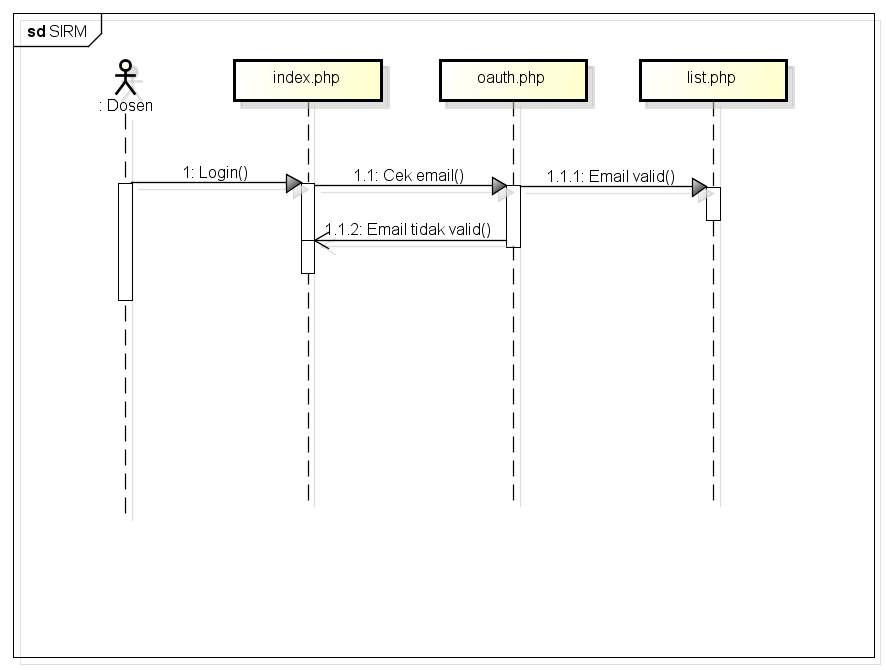
\includegraphics[scale=0.6]{Gambar/sekuenslogin.png}
%\caption[Diagram Sekuens Bagian Satu]{Diagram Sekuens Bagian Satu} 
%\label{fig:ds1}
%\end{figure}

%\begin{figure}[p]
%\centering
%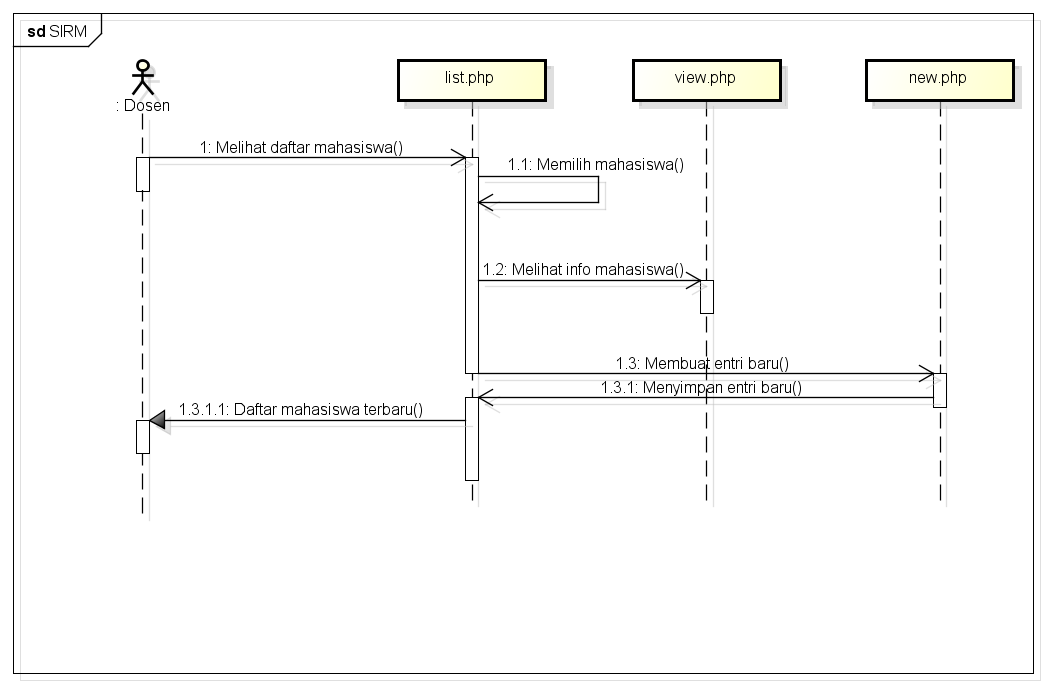
\includegraphics[scale=0.6]{Gambar/sekuenslist.png}
%\caption[Diagram Sekuens Bagian Dua]{Diagram Sekuens Bagian Dua} 
%\label{fig:ds2}
%\end{figure}

%\begin{figure}[pt]
%\centering
%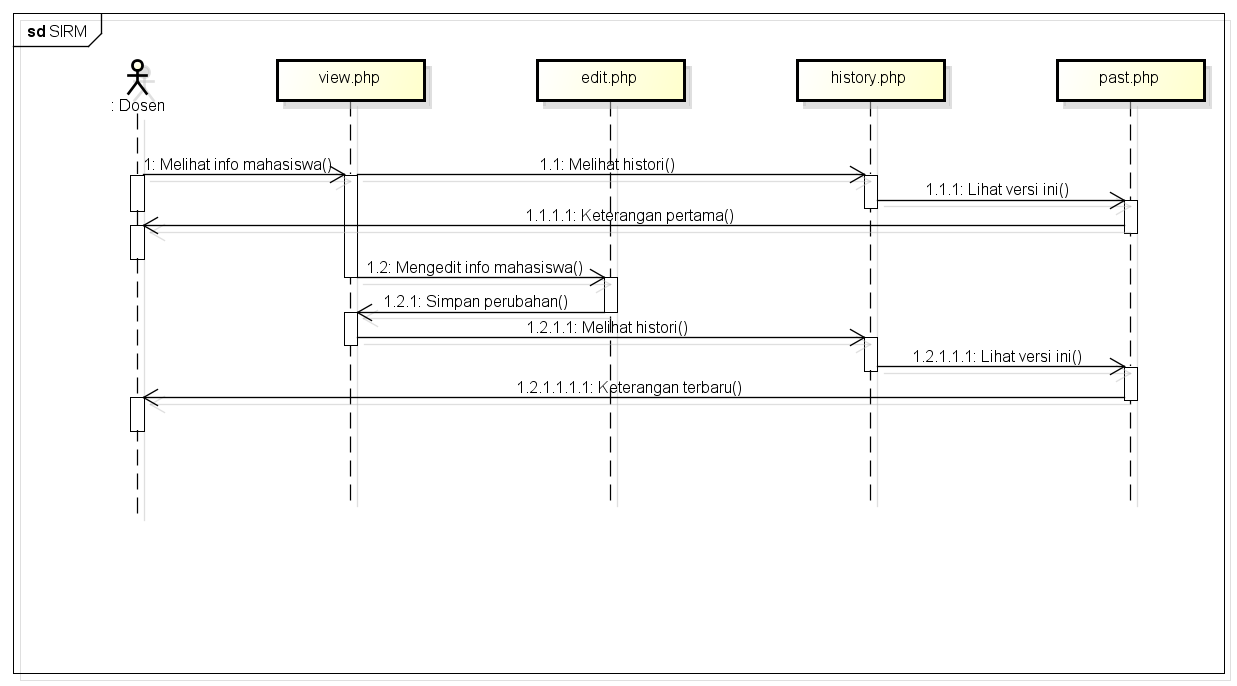
\includegraphics[scale=0.5]{Gambar/sekuensview.png}
%\caption[Diagram Sekuens Bagian Tiga]{Diagram Sekuens Bagian Tiga} 
%\label{fig:ds3}
%\end{figure}